\section{Introducción}
En este informe se describe todas las fases del desarrollo de un proyecto para la asignatura Taller de Proyecto 1. El proyecto consiste en el diseño y desarrollo de un sistema de cartel luminoso cuyo contenido es configurable de forma remota. El cartel tiene conectividad WiFi, con lo que es capaz de formar parte de una red IP.

No se tiene como objetivo realizar un producto diseñado de manera que sea economicamente viable producirlo en masa, sino más bien el desarrollo de un prototipo a modo de prueba de concepto.

El proyecto utilizó un proceso de desarrollo de cascada, como se muestra en la figura \ref{fig:waterfall}.

\begin{figure}[!htbp]
	\centering
	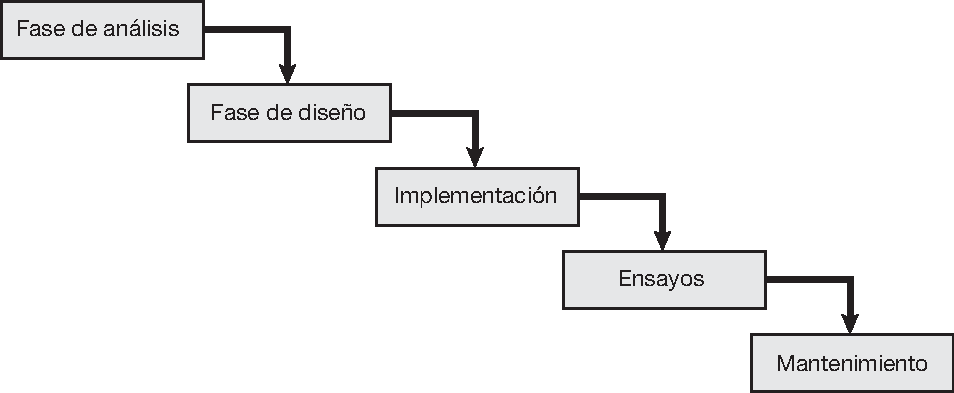
\includegraphics[width=\linewidth]{imagenes/waterfall.pdf}
	\caption{Modelo en cascada de desarrollo.}
	\label{fig:waterfall}
\end{figure}

A lo largo de este informe se documentarán las fases de desarrollo previamente mencionadas.

En la sección \ref{part:analisis} se habla sobre los requerimientos y especificaciones del sistema, detallando que funcionalidades debe tener y a cuáles restricciones está sujeto.

Luego, en la sección \ref{part:diseno}, se mencionan las componentes que constituyen el sistema, se explicitan modelos que describen el comportamiento del sistema, la interfaz de usuario y la arquitectura del software. También se muestran los esquemáticos que especifican la conexión de los componentes.

En la sección de implementación se documenta como se fue dando el proceso de desarrollo de software y la implementación física del hardware.

En la sección de ensayos se documenta los resultados de las pruebas que se realizaron sobre el sistema en funcionamiento.

Por ultimo, se anexa como apéndice una guía instructiva que explica los pasos necesarios para poner en marcha el sistema.

\part{Fase de análisis}\label{part:analisis}
\section{Requerimientos}
\section{Especificaciones}
\section{Software}
\subsection{Diseño de alto nivel}
\subsection{Diseño de bajo nivel}
\section{Hardware}
\part{Diseño}\label{part:diseno}
\part{Implementación}\label{part:impl}
\part{Ensayos y mediciones}\label{part:ensayos}